\section{Dominios en el desarrollo de sistemas mecatrónicos}

\subsection{Dominio lógico o funcional: funciones, relación, comportamiento}

Es el dominio donde se lleva a cabo la descomposición de funciones, la función principal que el sistema debe realizar es dividida en funciones que busquen definir y describir el comportamiento del sistema. Así mismo, deben cumplir los objetivos de diseño, los requerimientos y las necesidades. 

El dominio puede dividirse en \( m \) espacios, de acuerdo a los niveles jerárquicos de funciones

\begin{figure}[h!]
    \centering
        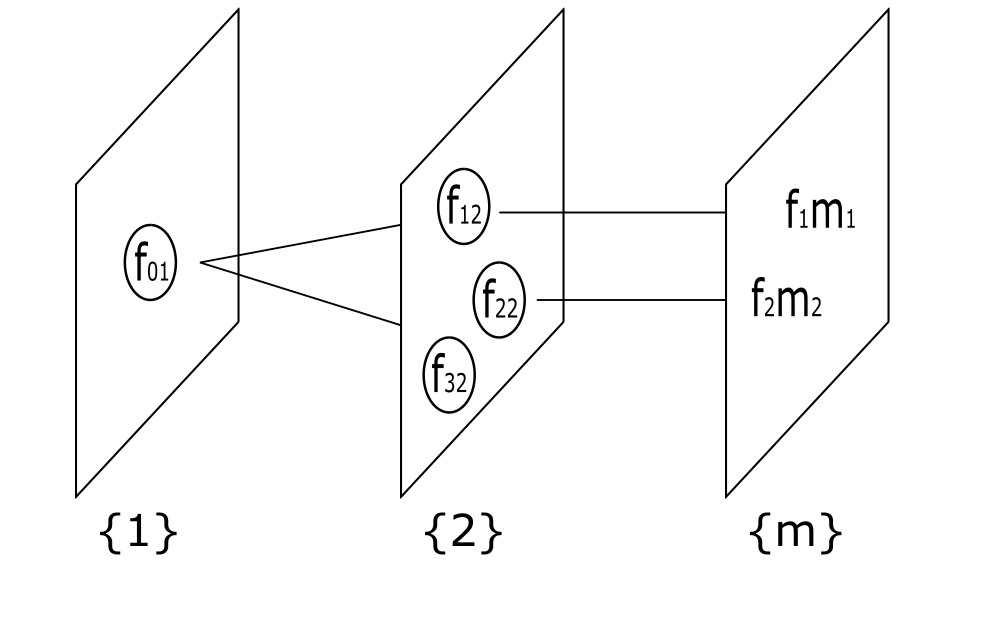
\includegraphics[scale=0.15]{Proyecto Integrador Figuras/11 dominio funcional.png}
        \caption{Dominio funcional}
\end{figure}

Una función puede definirse de manera general como la transformación de una entrada en una salida. Esta transformación debe mantener el índice de desempeño deseado. Las entradas y salidas de la transformación deben ser del tipo
\begin{enumerate}
    \item Materia
    \item Energía
    \item Información
\end{enumerate}

\subsection{Clasificación de funciones}
Las funciones se puede clasificar en los siguientes tipos
\begin{enumerate}
    \item Función principal: Es una parte fundamental del sistema, es lo que cumple el comportamiento del sistema. Es predominante independiente. A partir de esta función, se puede definir las funciones propias del sistema. 
    
    \item Funciones secundarias: Son las funciones requeridas para que el sistema cumpla con la función principal.
    
    \item Funciones básicas: Son funciones que un sistemas mecatrónico debe desempeñar, sin importar los objetivos de diseño, necesidades y requerimientos.
    
    \item Funciones irrealizables: Son funciones que debido a fenómenos físicos o tecnología actual no pueden realizarse.
\end{enumerate}

La descomposición de funciones se debe realizar de una forma jerárquica y sistematizada. Se recomienda que cada nivel (espacio) contenga las funciones que permitan describir el comportamiento del sistema. El proceso de descomposición es iterativo.

\subsection{Relación entre funciones}

La interrelación entre funciones está definida por la conexión y la comunicación de las entradas y salidas, describiendo en conjunto el comportamiento del sistema.

Se puede definir una función de manera general como:

\[
    \mathcal{F}: A(E, M, I) \to B(E, M, I)
\]

Donde \( \mathcal{F} \) es la función que transforma las entradas de \( A \) en las salidas de \( B \).

Cuando una función está compuesta de dos funciones (f1, f2), la relación entre ellas se puede definir como:
\begin{enumerate}
    \item Si la trayectoria de \( f_{1} \) está contenida en \( f_{2} \) se considera que las funciones son secuenciales. Se puede definir la relación como la composición de funciones \( (f_{1} o f_{2}) \). Las salidas de \( f_{1} \) se convierten en las entradas de \( f_{2} \).
        
    \begin{figure}[h!]
        \centering
            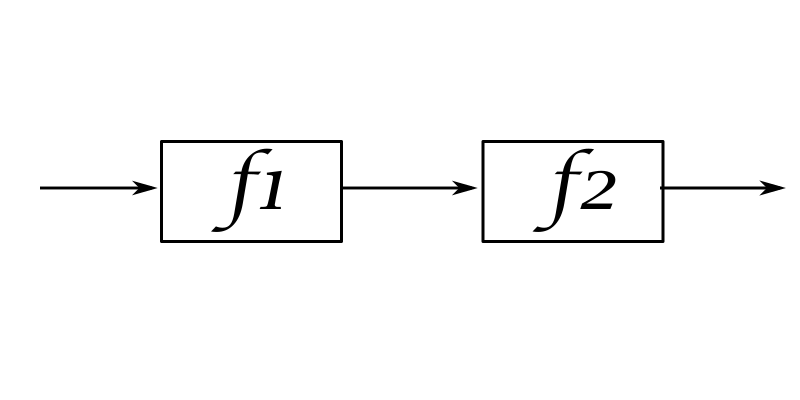
\includegraphics[scale=0.25]{Proyecto Integrador Figuras/12 Funcion Secuencial.png}
            \caption{Ciclo de vida de proyecto}
     \end{figure}
        
    \item Si la trayectoria de cada función es independiente, entonces las funciones son paralelas y su transformación puede ser simultanea. El operador "AND" se emplea para describir esta operación.
    
    \begin{figure}[h!]
        \centering
            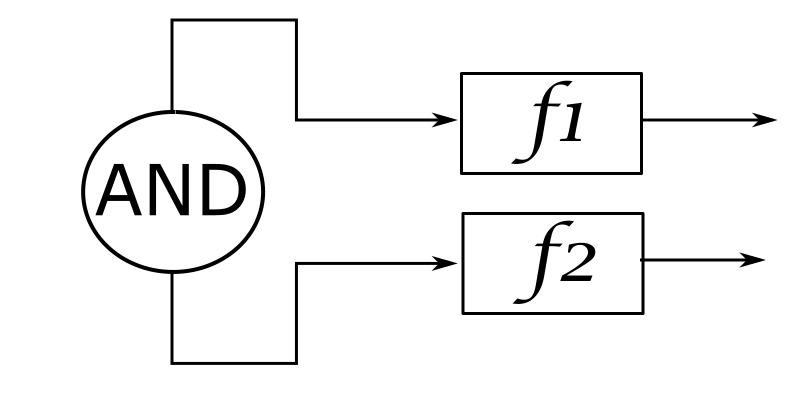
\includegraphics[scale=0.25]{Proyecto Integrador Figuras/13 Funcion AND.png}
            \caption{Ciclo de vida de proyecto}
     \end{figure}
    
    \item Si la trayectoria de cada función es independiente, son paralelas, pero no pueden realizar la transformación simultánea. Se emplea el operador "XOR".
    
    \begin{figure}[h!]
        \centering
            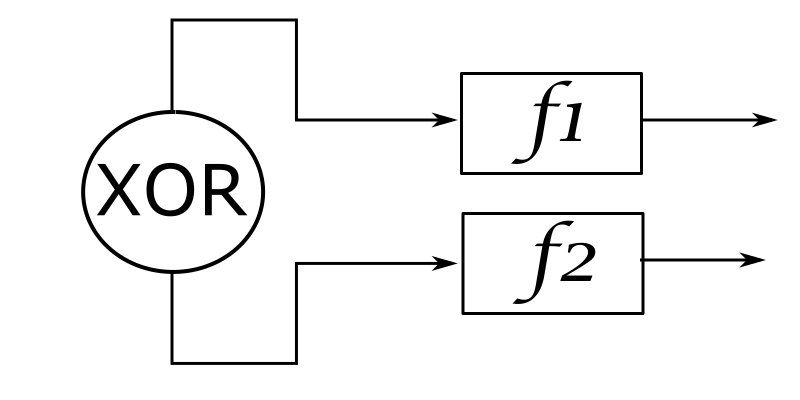
\includegraphics[scale=0.25]{Proyecto Integrador Figuras/14 Funcion XOR.png}
            \caption{Ciclo de vida de proyecto}
     \end{figure}
\end{enumerate}